\documentclass{beamer}

\usetheme[hideothersubsections]{Berkeley}

% these are typical

\usepackage{latexsym}		% to get LASY symbols
\usepackage{epsfig}		% to insert PostScript figures
\usepackage{graphicx}           % to insert any other kind of figure

% these are for math stuff

\usepackage{amsmath}	% AMS math features (e.g., eqn alignment)
\usepackage{amssymb}	% Various weird symbols
\usepackage{amsfonts}	% Various useful math fonts
\usepackage{amsthm}	% Fancy theorem-type environments

% Uncomment these lines to make full-size pages for printing
%\usepackage{pgfpages}
%\pgfpagesuselayout{resize to}[letterpaper,border shrink=5mm,landscape]

% {definition}, {example}, {examples}, {lemma}, {theorem}, and {fact}
% already defined
\newtheorem{question}{Question}
\newtheorem{conjecture}{Conjecture}

\begin{document}

\raggedright

\title{A Question Answering System Using Encoder-decoder Sequence-to-sequence Recurrent Neural Networks}
\author{Bo Li}
\date{May 11, 2018}
\institute[SJSU]{San Jos\'{e} State University}

\begin{frame}
\titlepage

\end{frame}

\begin{frame}

  \frametitle{Outline}

  \tableofcontents[hideallsubsections]

\end{frame}



\section{Introduction}

\begin{frame} \frametitle{Topic of This Project}
    \begin{itemize}
        \item Question answering is the study of writing computer programs that can answer natural language questions.
        \item In this project, we focused on a scenario where a specific passage is already assigned to a question and the answer is a segment of the passage.
        \item Stanford Question Answering Dataset (SQuAD) is suitable for such scenario. It is used in this project.
        \begin{itemize}
            \item It includes questions asked by human beings on Wikipedia articles.
            \item The answer to each question is a segment of the corresponding Wikipedia passage
            \item It contains more than 100,000 question-answer pairs on more than 500 articles.
        \end{itemize}


    \end{itemize}
\end{frame}

\begin{frame}{An example}
    \begin{examples}
            \begin{itemize}
                \item Passage: The city had a population of 1,307,402 according to the 2010 census , distributed over a land area of 372.1 square miles ( 963.7 km2 ) . The urban area of San Diego extends beyond the administrative city limits and had a total population of 2,956,746 , making it the third-largest urban area in the state , after that of the Los Angeles metropolitan area and San Francisco metropolitan area . They , along with the Riverside–San Bernardino , form those metropolitan areas in California larger than the San Diego metropolitan area , with a total population of 3,095,313 at the 2010 census .
                \item Question: How many square miles does San Diego cover ?
                \item Answer: 372.1
            \end{itemize}
        \end{examples}
\end{frame}

\begin{frame}{Technique Used in This Project}
The encoder-decoder sequence-to-sequence recurrent neural networks were used in this project.
   \begin{itemize}
       \item Encoder-decoder:  encode an input to some vectors and then decode those vectors to an output.
       \item Sequence-to-sequence: Input is a sequence; output is also a sequence
            \begin{itemize}
                \item For question answering, the input sequence includes a passage and a question and the output sequence is the answer
            \end{itemize}
       \item Recurrent Neural Networks: Networks used for modeling sequential data

   \end{itemize}
\end{frame}

\begin{frame}{Contribution of This Project}
    \begin{itemize}
        \item We successfully built a question answering system using an existing model and four models that were designed by making changes to the existing model.
        \item By comparing the results of five different models, we got two interesting observations. We will give details in Experiments part.
    \end{itemize}
\end{frame}

\section{Background}

\begin{frame} \frametitle{Word Feature Vector}
  \begin{examples}
  An example from the GloVe word feature vectors.
    \begin{itemize}
        \item Word: the
        \item Word feature vector: [0.418 0.24968 -0.41242 0.1217 0.34527 -0.044457 -0.49688 -0.17862 -0.00066023 -0.6566 0.27843 -0.14767 -0.55677 0.14658 -0.0095095 0.011658 0.10204 -0.12792 -0.8443 -0.12181 -0.016801 -0.33279 -0.1552 -0.23131 -0.19181 -1.8823 -0.76746 0.099051 -0.42125 -0.19526 4.0071 -0.18594 -0.52287 -0.31681 0.00059213 0.0074449 0.17778 -0.15897 0.012041 -0.054223 -0.29871 -0.15749 -0.34758 -0.045637 -0.44251 0.18785 0.0027849 -0.18411 -0.11514 -0.78581]
    \end{itemize}
  \end{examples}
\end{frame}


\begin{frame}{Word Feature Vector, cont.}
\begin{itemize}
      \item A word feature vector represents a word according to its relationship with other words in a vocabulary.
      \item The word feature vectors for the vocabulary of a given text are learned by training a neural probabilistic language model on the text.
      \item In practice, in neural network models for natural language processing, word feature vectors are used to represent words. This is how we use word feature vector in this project.
  \end{itemize}
\end{frame}



\begin{frame}{Recurrent Neural Networks}

    \begin{itemize}
        \item Recurrent Neural Networks (RNNs) are used for modeling sequential data.
        \item In practice, due to vanishing problem, more complex learning unit such as Long Short Term Memory (LSTM) cell or Gated Recurrent Unit (GRU) are used. In this project, we used LSTM and GRU equally as learning unit.
    \end{itemize}



\end{frame}



\begin{frame}{Recurrent Neural Networks, cont.}
    \begin{examples}{A recurrent network with no outputs for encoding process.}
        \begin{itemize}
            \item $x$ is the input. $h$ is the state. $\theta$ is the hyperparameter.
            \item The relation between $h$ and $x$ is $h_t = f(h_{t-1}, x_t; \theta).$
                \begin{center}
                  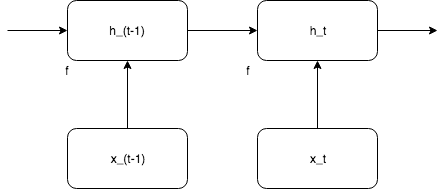
\includegraphics[width=5cm, height=2cm]{figures/rnnWithNoOutputs}
                \end{center}
            \item An example of $f$ is $h_t = sigmoid(W_h h_{t-1} + W_x x_t + b).$
            \item An example of input sequence $x_1, ..., x_n$ is the word feature vector sequence which corresponds to the word sequence ``How many square miles does San Diego cover ?''.
            \item An example of what we want after operating this RNN is $h_1, ..., h_n$.
        \end{itemize}
    \end{examples}
\end{frame}

\begin{frame}{Bidirectional Recurrent Neural Networks}
    \begin{itemize}
        \item Problem of RNNs: $h_t$ only contains context information from $x_1$ to $x_t$
        \item Solution given by Bidirectional RNNs:
            \begin{itemize}
                \item one cell operates from left to right, and another cell operates from right to left
                \item using both $h_t$ and $g_t$ can get context information of the whole sequence
            \end{itemize}
             \begin{center}
                  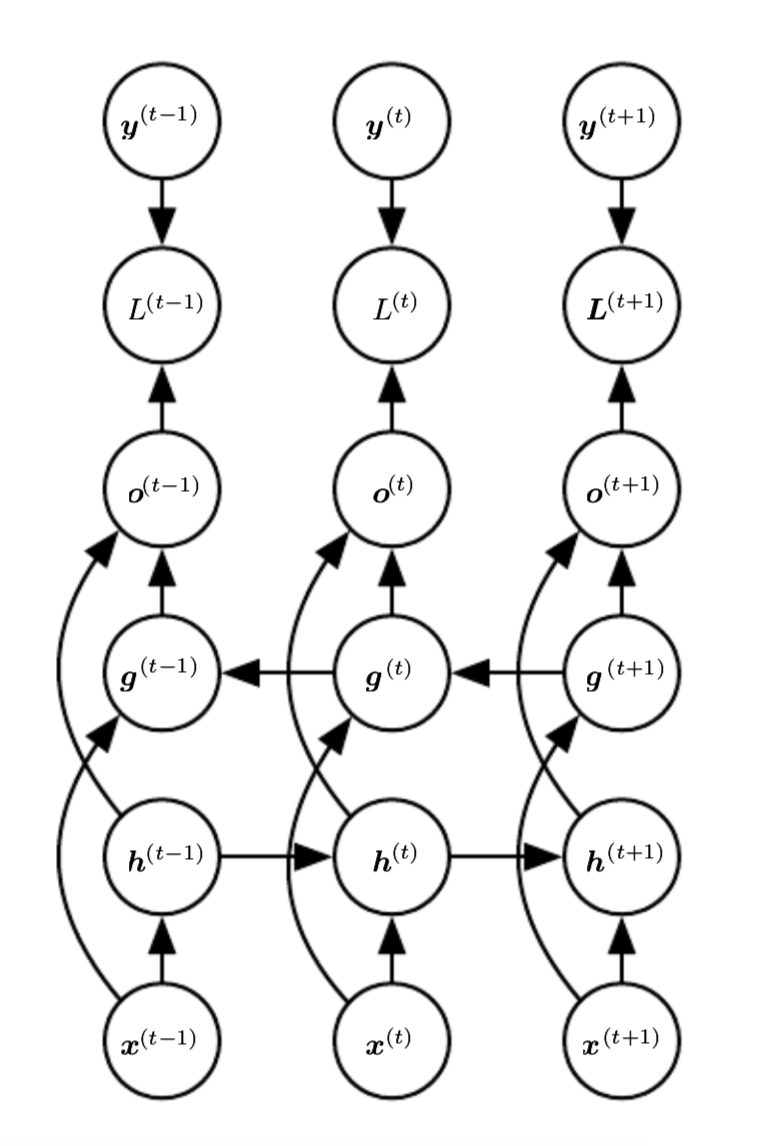
\includegraphics[width=8cm, height=4cm]{figures/bidirectionalRnn.png}
            \end{center}
    \end{itemize}
\end{frame}

\begin{frame}{Bidirectional Recurrent Neural Networks}
    \begin{itemize}
        \item In this project, we used bidirectional RNNs in encoding part. But for simplicity in presentation, I might talk about RNNs instead of Bidirectional RNNs in some parts.

    \end{itemize}
\end{frame}

\begin{frame}{Encoder-decoder Sequence-to-sequence Architecture}
\begin{itemize}
    \item The process of understanding the input sequence is considered as encoding the input sequence to some vectors $Crypto$.
    \item The process of generating output is considered as decoding the $Crypto$.
\end{itemize}



\end{frame}

\begin{frame}{Encoder-decoder Sequence-to-sequence Architecture, Cont.}
\begin{examples}
$x$ is the input, $h$ is the state in encoding process, $y$ is the output, and $g$ is the state of decoding process.
\begin{center}
        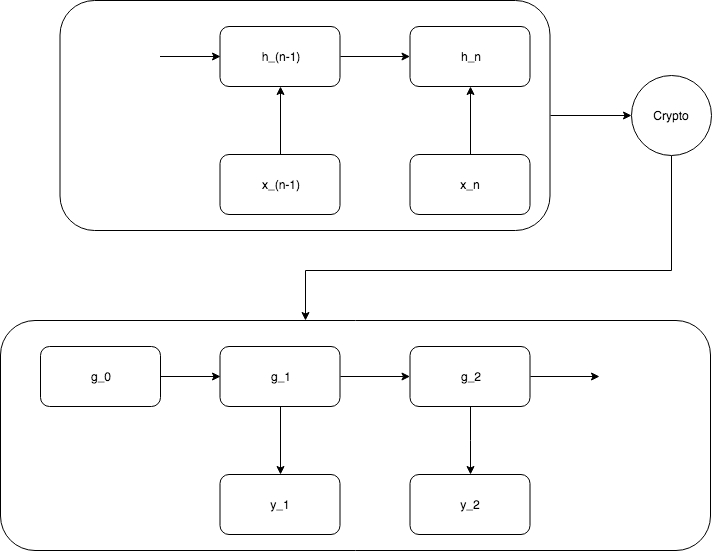
\includegraphics[width=8cm, height=5cm]{figures/encoderDecoder.png}
    \end{center}
\end{examples}

\end{frame}

\begin{frame}{Encoder-decoder Sequence-to-sequence Architecture, Cont.}
    \begin{itemize}
        \item In this project, each input sequence actually includes two sequences - a question and a passage.
            \begin{itemize}
                \item Attention mechanism is required to make each passage aware of the corresponding question.
            \end{itemize}
        \item In this project, each output sequence is an answer which is represented by two indices for the input passage sequence.
            \begin{itemize}
                \item The pointer network is used to make sure the output sequence comes from input sequence.
            \end{itemize}
    \end{itemize}
\end{frame}

\begin{frame}{Attention Mechanism}
    \begin{itemize}
        \item Intuitively, attention mechanism is one way to pay attention to a sequence of vectors.
        \item The key to understand attention mechanism is to understand how to get attention weight vector $\alpha$.
        \item Using the attention weight vector $\alpha$, we can get a weighted average of the sequence of vectors. This weight average is called attention vector.
    \end{itemize}
    \begin{examples}
    How attention mechanism was used in neural machine translation. In this scenario, the sequence of vectors to pay attention to is the encoding states.
        \begin{itemize}
            \item $y$ is the output, $g$ is the state, and $c$ is the attention vector. $$g_i =f(g_{i-1},y_{i-1},c_i).$$

        \end{itemize}
    \end{examples}
\end{frame}

\begin{frame}{Attention Mechanism, cont.}
    \begin{examples}
     \begin{center}
        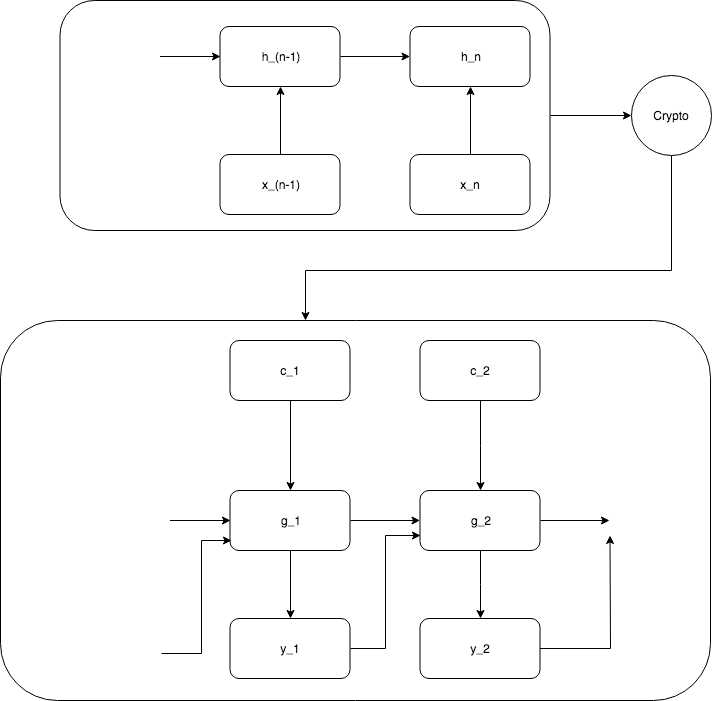
\includegraphics[width=7cm, height=6cm]{figures/attention}
    \end{center}
    \end{examples}
\end{frame}

\begin{frame}{Attention Mechanism, cont.}
    \begin{examples}
        \begin{itemize}
            \item The attention vector $c_i$ is produced by using $g_{i-1}$ to ``query'' the encoding states $h_1, ... h_n$ through
        $$c_i = \sum _j {\alpha _{i,j} h_j}$$
        $$\alpha _{i,j} = \exp{e_{i,j}} / \sum _j {\exp{e_{i,j}}}$$
        $$e_{i,j} = tanh(W_h h_j + W_g g_{i-1} + b).$$
        \end{itemize}
    \end{examples}
\end{frame}


\begin{frame}{Attention Mechanism, cont.}
    \begin{itemize}
        \item In this project, the attention mechanism is used in both encoding and decoding part.
        \item In the encoding part, each word feature vector in passage pays attention to the corresponding question word feature vector sequence.
        \item In the decoding part, each decoding state pays attention to the sequence encoding states.
    \end{itemize}






\end{frame}

\begin{frame}{Pointer Network}
    \begin{itemize}
        \item Using the pointer network enables the decoder to output tokens from input sequence.
        \item In this project, the pointer network was used in the decoding part which generates the answer.
        \item The attention weight vector $\alpha$ is considered as a probability distribution which indicates how likely each token in the input sequence is the current output token.
    \end{itemize}
\end{frame}

\begin{frame}{Pointer Network, cont.}
    \begin{examples}
        $y_i = x_k$ where $k = argmax_j(\alpha _{i,j}).$
        \begin{center}
            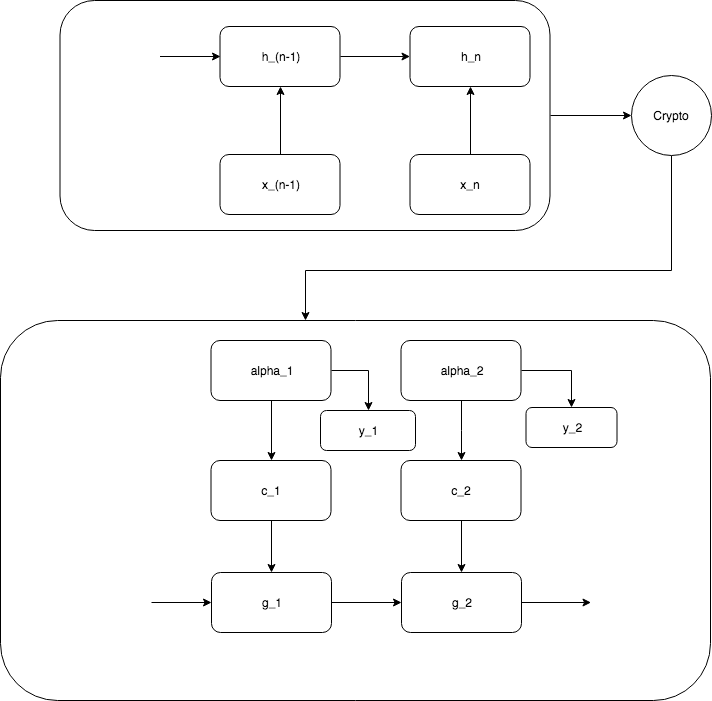
\includegraphics[width=8cm, height=6cm]{figures/pointerNetwork.png}
        \end{center}
    \end{examples}


\end{frame}


\section{Design}

\begin{frame}{Relationship Between Five Different Models}
    \begin{itemize}
        \item Model 1 is the Match LSTM \& Answer Pointer model designed by Wang and Jiang.
        \item Model 2, 3, 4 and 5 are designed by us through making changes to Model 1.
    \end{itemize}
\end{frame}

\begin{frame} \frametitle{Model 1}\framesubtitle{Overview}
  \begin{itemize}
      \item Model 1 has an encoder-decoder sequence-to-sequence architecture.
      \item Model 1 is trained on SQuAD dataset.
            \begin{itemize}
                \item Each instance of training data includes one passage, one question and one answer.
                \item The passage is a sequence of tokens.
                \item The question is a sequence of tokens.
                \item The answer is a sequence of two indices indicating the start and end positions in passage.
            \end{itemize}
      \item Before feeding training data into the model, tokens are converted to word feature vectors.
  \end{itemize}
\end{frame}

\begin{frame} \frametitle{Model 1, cont.}\framesubtitle{Structure}
    \begin{itemize}
        \item Encoder
            \begin{itemize}
                \item the preprocessing layer
                \item the bidirectional match LSTM layer
            \end{itemize}
        \item Decoder
            \begin{itemize}
                \item the answer pointer layer
            \end{itemize}
    \end{itemize}

\end{frame}

\begin{frame} \frametitle{Model 1, cont.}\framesubtitle{Structure}
    \begin{center}
        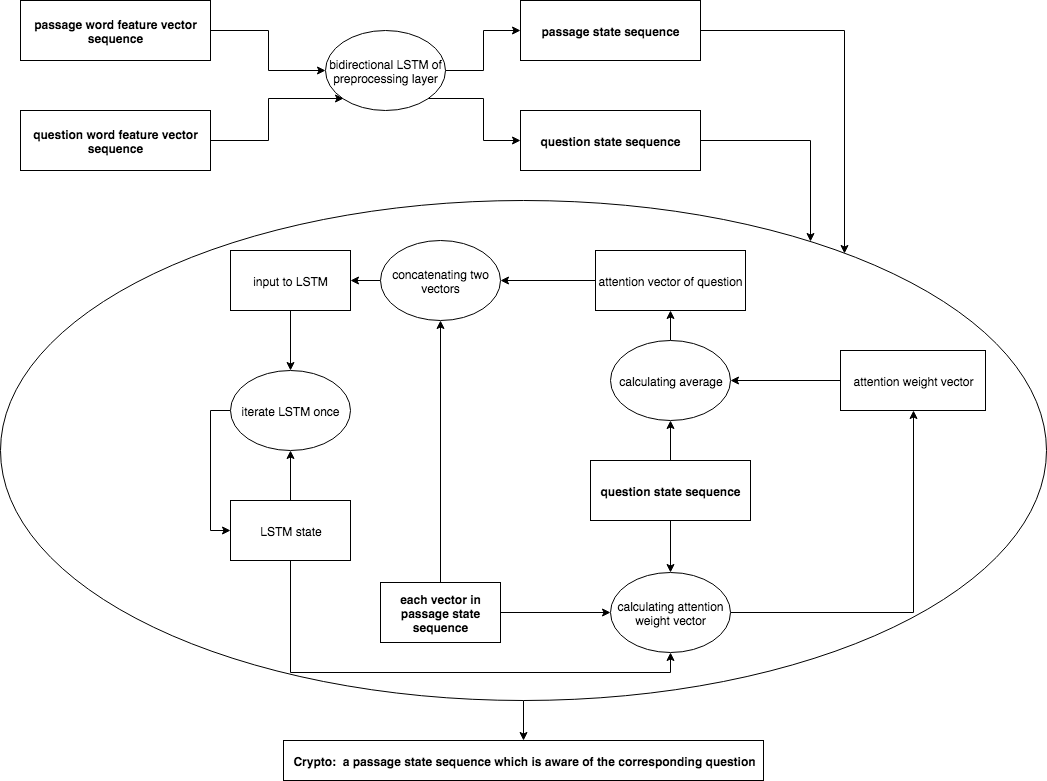
\includegraphics[width=10cm, height=7cm]{figures/model1_encoder.png}
    \end{center}
\end{frame}

\begin{frame} \frametitle{Model 1, cont.}\framesubtitle{Structure}
    \begin{center}
        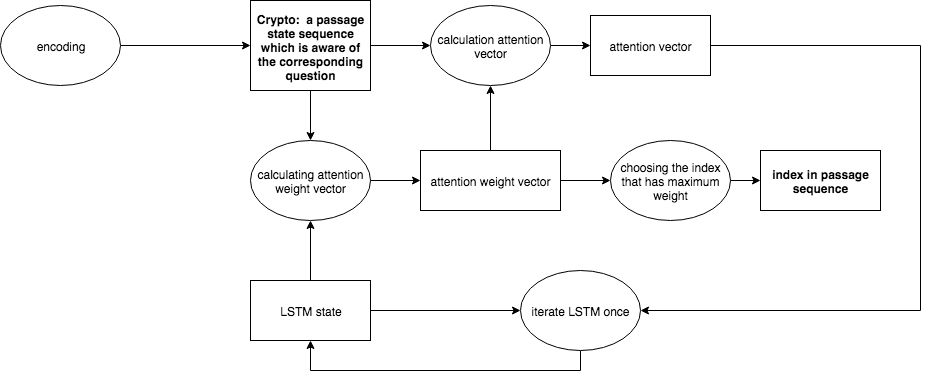
\includegraphics[width=10cm, height=5cm]{figures/model1_decoder.png}
    \end{center}
\end{frame}

\begin{frame} \frametitle{Model 1, cont.}\framesubtitle{The Preprocessing Layer}

    \begin{itemize}
        \item A LSTM runs over each passage word feature vector sequence and outputs a sequence of LSTM states
        \item The same LSTM is used to encode each question word feature vector sequence to a sequence of LSTM states.
    \end{itemize}
\end{frame}

\begin{frame} \frametitle{Model 1, cont.}\framesubtitle{The Preprocessing Layer}
    $$H^p = \overrightarrow{LSTM}(P)$$
    $$H^q = \overrightarrow{LSTM}(Q)$$

    where

    $$P\in R^{d \times p}: passage$$
    $$Q\in R^{d \times q}: question$$
    $$H^p\in R^{l \times p}: encoded\ passage$$
    $$H^q\in R^{l \times q}: encoded\ question$$
    $$p: length \ of\ passage$$
    $$q: length\ of\ question$$
    $$l: dimension\ of\ LSTM\ states$$
    $$d: dimension\ of\ word\ feature\ vector$$

\end{frame}

\begin{frame} \frametitle{Model 1, cont.}\framesubtitle{The Bidirectional Match LSTM Layer}
    \begin{itemize}
        \item Match LSTM: A LSTM equipped with the attention mechanism
        \item The match LSTM encodes each passage state sequence and the corresponding question state sequence into match LSTM state sequence.
    \end{itemize}
\end{frame}

\begin{frame} \frametitle{Model 1, cont.}\framesubtitle{The Bidirectional Match LSTM Layer}

    $$\overrightarrow{G} = tanh(W^qH^q + (W^p{h_i}^p + W^r\overrightarrow{{h_{i-1}}^r} + b^p) \otimes e_q)$$
    $$\overrightarrow{\alpha _i} = softmax(w^t\overrightarrow{G_i} + b \otimes e_q)$$


    where

    $$W^q, W^p, W^r\in R^{l \times l} $$
    $$b_p, w\in R^{l}  $$
    $$b \in R $$
    $${h_{i}^p}\in R^{l}: one\ column\ of\ H^p  $$

    and

    \[ \overrightarrow{z_i} =
    \begin{bmatrix}
    {h_i}^p \\
    H^q\overrightarrow{ {\alpha _i}}^T \\
    \end{bmatrix}
    \in R^{2l}
    \]
    $$\overrightarrow{{h_i}^r} = \overrightarrow{LSTM}(\overrightarrow{z_i}, \overrightarrow{{h_{i-1}}^r}).$$

\end{frame}

\begin{frame} \frametitle{Model 1, cont.}\framesubtitle{The Bidirectional Match LSTM Layer}
    \begin{itemize}
        \item After iterating between getting attention weight vector $\overrightarrow{\alpha _i}$ and getting match LSTM state ${{h_{i}}^r}$ $p$ times, we get $[{{h_{1}}^r}, ..., {{h_{p}}^r}]$. Concatenate them to get

        $$\overrightarrow{H^r} = [{{h_{1}}^r}, ..., {{h_{p}}^r}] \in R^{l \times p}.$$

        \item Then go over $H^p$ from right to left to get $\overleftarrow{H^r}$. Concatenate $\overrightarrow{H^r}$ and $\overleftarrow{H^r}$ to get the final output of encoding process

        \[ H^r =
        \begin{bmatrix}
        \overrightarrow{H^r} \\
        \overleftarrow{H^r} \\
        \end{bmatrix}
        \in R^{2l \times p}.
        \]
    \end{itemize}

\end{frame}

\begin{frame} \frametitle{Model 1, cont.}\framesubtitle{The Answer Pointer Layer}
    \begin{itemize}
        \item Each output of the decoding process includes two probability distributions.
           \begin{itemize}
               \item The first probability distribution tells how likely each token in passage to be the start of the answer.
               \item The second probability distribution tells how likely each token in passage to be the end of the answer
           \end{itemize}
    \end{itemize}

\end{frame}

\begin{frame}\frametitle{Model 1, cont.}\framesubtitle{The Answer Pointer Layer}
    \begin{itemize}
        \item The answer LSTM decodes match LSTM states to the two probability distributions.
        $$F_k = tahn(VH^r + (W^a{h^a_{k-1}} +  b^a) \otimes e_p)$$
        $$\beta _k = softmax(v^tF_k + c \otimes e_p)$$


        where
        $$V \in R^{l \times 2l}$$
        $$W^a\in R^{l \times l} $$
        $$b_a, v\in R^{l}  $$
        $$c \in R $$
        $${h_{k-1}}^a\in R^{l}: ith\ state\ of\ answer\ LSTM  $$

        and


        $${h_k}^a = LSTM(H^r\beta _k^T, h_{k-1}^a)$$
    \end{itemize}
\end{frame}

\begin{frame}\frametitle{Model 1, cont.}\framesubtitle{The Answer Pointer Layer}
    \begin{itemize}
        \item By iterating two times, we could get the output of the decoding process - $\beta _0$ and $\beta _1$.
    \end{itemize}

\end{frame}

\begin{frame}\frametitle{Model 1, cont.}\framesubtitle{loss function}
    \begin{itemize}
        \item Let $a_s$ denote the ground truth start index of the answer and $a_e$ denote the ground truth end index, we have

        $$p(a|H^r) = p(a_s|H_r)p(a_e|H_r)=\beta _{0, a_s} \times \beta_{1, a_e}$$

        where $$\beta_{k, j} = jth\ token\ of\ \beta _k$$
        \item To train the model, the loss function

        $$J(\theta) = -\frac{1}{N}\sum_{i=1}^{N} \log{p(a^n|H^r)} $$

        is minimized.

    \end{itemize}

\end{frame}

\begin{frame} \frametitle{Model 2}
    The difference from Model 2 and Model 1 is in the decoding process. In Model 2,
    $${h_k}^a = H^r\beta _{k}^T.$$
    That is, instead of the current state of answer LSTM, the previous attention vector is used to query the current attention weight vector.
\end{frame}


\begin{frame}{Model 2, cont.}
    \begin{center}
        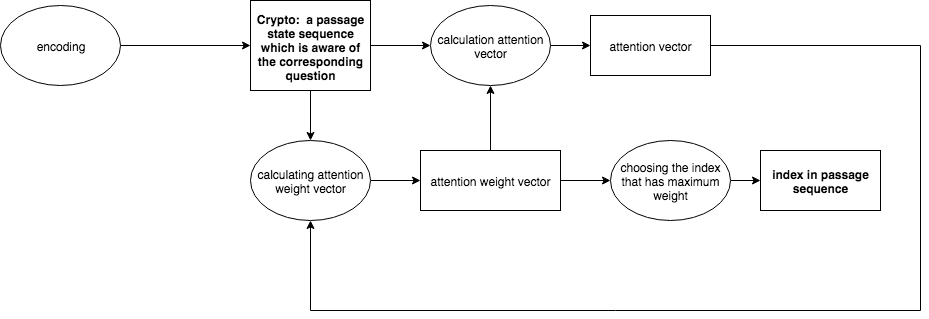
\includegraphics[width=10cm, height=5cm]{figures/model2_decoder.png}
    \end{center}
\end{frame}



\begin{frame} \frametitle{Model 3}
    The difference between Model 3 and Model 2 is that in Model 3 the $W^r\overrightarrow{{h_{i-1}}^r}$ in the bidirectional match LSTM layer is removed. This modification aims at checking whether $\overrightarrow{{h_{i-1}}^r}$ carries some redundant context information. After this change,


    $$\overrightarrow{G} = tanh(W^qH^q + (W^p{h_i}^p + b^p) \otimes e_q)$$
\end{frame}

\begin{frame}{Model 3, cont.}
    \begin{center}
        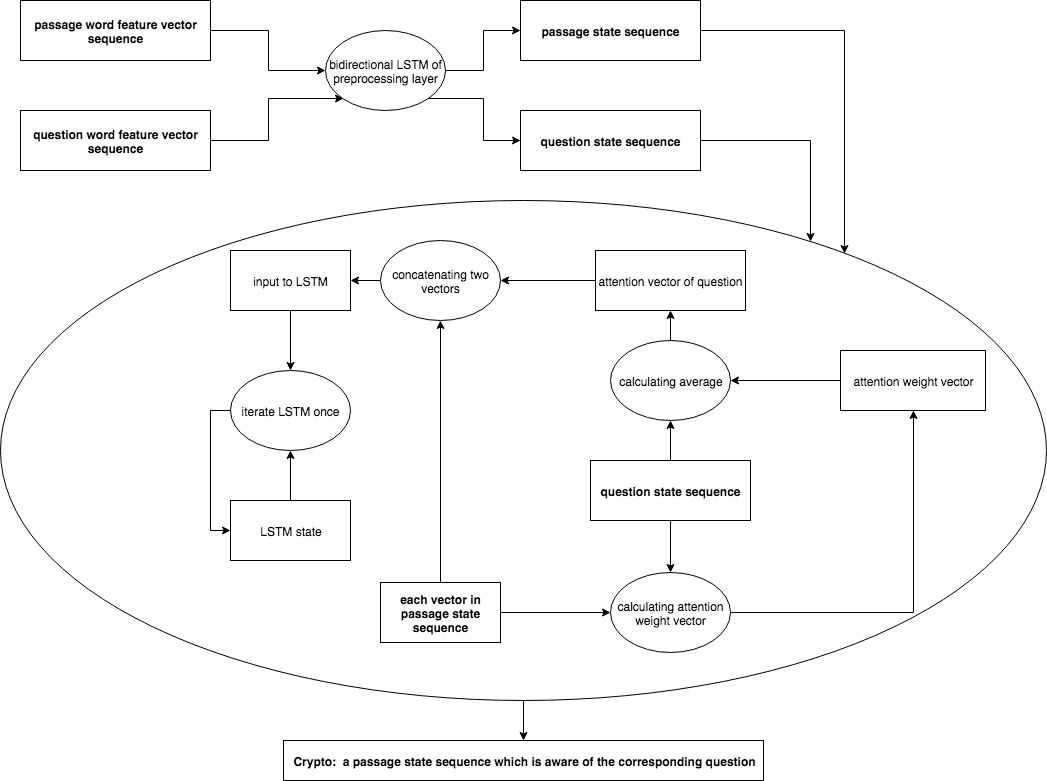
\includegraphics[width=10cm, height=7cm]{figures/model3_encoder.png}
    \end{center}
\end{frame}

\begin{frame} \frametitle{Model 4}
    The difference between Model 4 and Model 2 is that in Model 4 the the preprocessing layer is removed. This modification aims at checking whether the preprocessing layer carries some redundant context information.
\end{frame}

\begin{frame}{Model 4, cont.}
    \begin{center}
        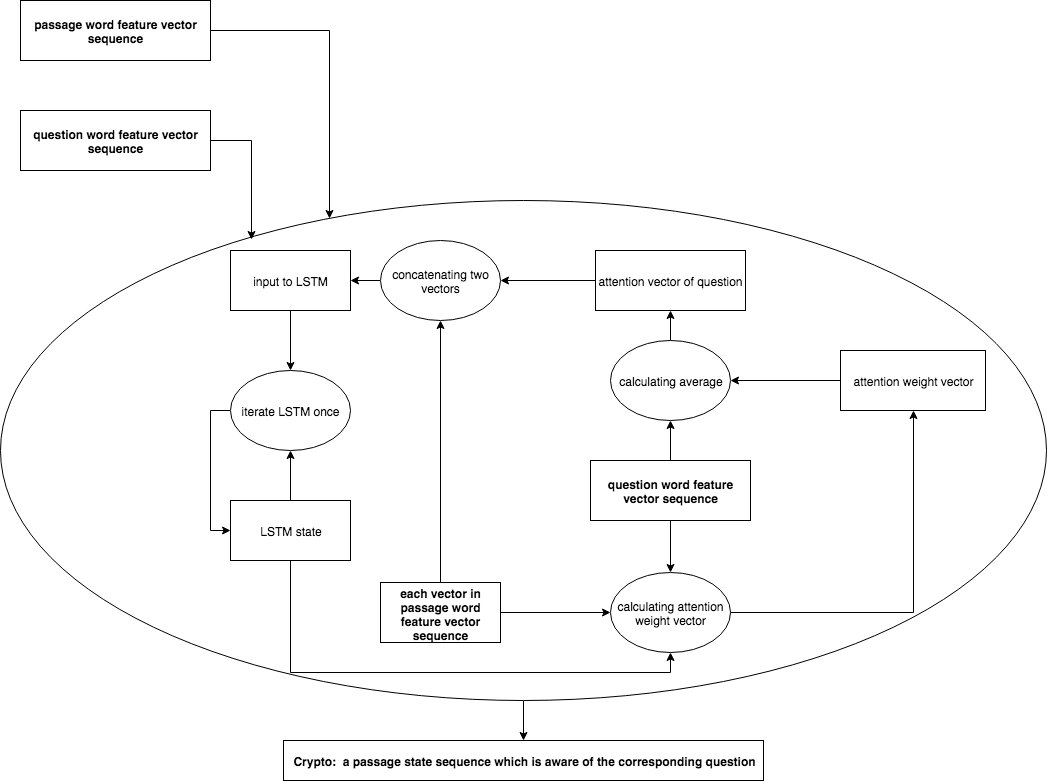
\includegraphics[width=10cm, height=7cm]{figures/model4_encoder.png}
    \end{center}
\end{frame}

\begin{frame} \frametitle{Model 5}
    The difference between Model 5 and Model 2 is that in Model 5 both the preprocessing layer and $W^r\overrightarrow{{h_{i-1}}^r}$ in the bidirectional match LSTM layer are removed. This aims at checking whether context information carried by both is included in some other parts of Model 2.
\end{frame}


\begin{frame}{Model 5, cont.}
    \begin{center}
        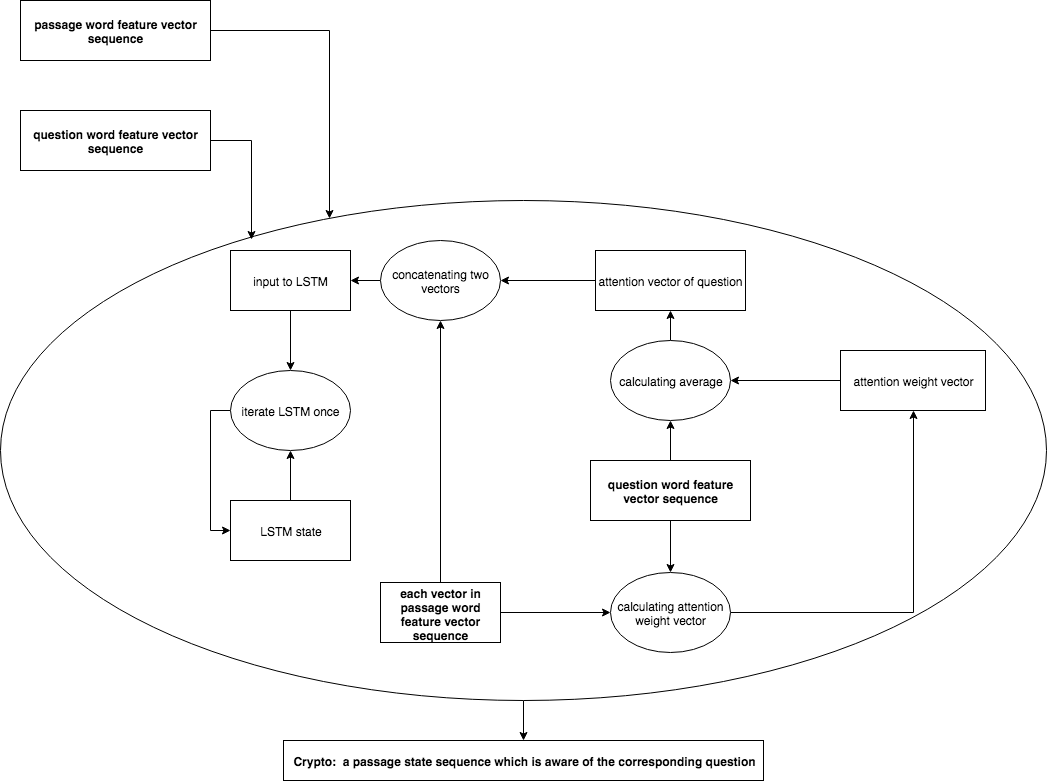
\includegraphics[width=10cm, height=7cm]{figures/model5_encoder.png}
    \end{center}
\end{frame}

\section{Implementation}

\begin{frame} \frametitle{Adjusting Models for Batch Training}\framesubtitle{Why necessary?}
    \begin{itemize}
        \item When training a model, all of the training data is fed into the model to update the parameters.
        \item In one specific model, the number of times to iterate the encoding process is fixed.
        \item However, different passages have different lengths and different questions also have different lengths.
        \item As such, adjusting all passages to a same length and adjusting all questions to another same length are necessary.
    \end{itemize}
\end{frame}

\begin{frame}\frametitle{Adjusting Models for Batch Training}\framesubtitle{How to pad?}
Take a passage as an example.
    \begin{itemize}
        \item Each passage is adjusted to $passage\_padding\_length$.
            \begin{itemize}
                \item For sequences longer than the fixed length, a part of the sentence is cut out.
                \item For sequences shorter than the fixed length, a faking pad token is used to pad them.
            \end{itemize}
        \item Each passage is paired with a mask vector $passage\_mask$ which has size $passage\_padding\_length$
            \begin{itemize}
                \item Each entry of mask vector is either zero or one. \item Zero indicates that the current token does not exist in the original sequence. One indicates the opposite.
            \end{itemize}
    \end{itemize}
\end{frame}

\begin{frame}\frametitle{Adjusting Models for Batch Training}\framesubtitle{How to Adjust Models?}
    \begin{itemize}
        \item In the preprocessing layer, after getting a sequence of states, the mask vector is used to reset the values of positions that do not exist to zero in an additional step
        $$H^p = H^p \circ (passage\_mask \otimes l)$$
        $$H^q = H^q \circ (question\_mask \otimes l).$$
        \item In the match LSTM layer, the attention weights of positions that do not exist are also set to zero in an additional step
        $$\overrightarrow{\alpha _i} = softmax( (w^t\overrightarrow{G_i} + b \otimes e_q) ) \circ question\_mask .$$
        Similar to the preprocessing layer, we have
        $$H_r = H_r \circ (passage\_mask \otimes 2l).$$
        \item In the answer pointer layer, we have
        $$\beta _k = softmax( (v^tF_k + c \otimes e_p) ) \circ passage\_mask.$$
    \end{itemize}
\end{frame}

\begin{frame}{Tensorflow Graphs}
    \begin{itemize}
        \item Tensorflow is an open source machine learning framework.
        \item The central idea of Tensorflow is describing a complex numeric computation as a graph.
        \item {\tt Variables} are ``trainable'' nodes.
        \item {\tt Placeholders} are nodes whose values are fed in run time.
    \end{itemize}
\end{frame}

\begin{frame}{Tensorflow Graphs}\framesubtitle{Taking Model 1 as an example}
     \begin{itemize}
         \item {\tt Variables} should be used to represent all the parameters of the encoding and decoding layers.
         \item {\tt Placeholders} should be used to represent passages, questions, and answers.
         \item To train a graph, some APIs of Tensorflow are called to get a train operation.
         \item Then the training data is fed through {\tt Placeholders} to run the train operation. When the train operation is run, the {\tt Variables} are updated.
     \end{itemize}
\end{frame}

\begin{frame}{Tensorflow Graphs}\framesubtitle{Taking Model 1 as an example}
    \begin{center}
        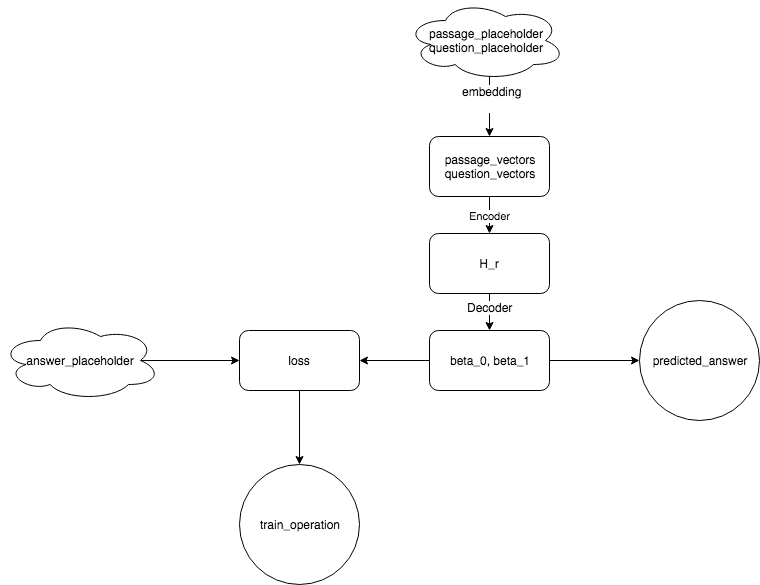
\includegraphics[width=8cm, height=6cm]{figures/tf_graph.png}
    \end{center}
\end{frame}

\begin{frame}{Implementation Pipeline}
    \begin{itemize}
        \item For a specific model, in the train and validation process, some Tensorflow graphs that have same structure but different values for {\tt Variables} are saved.
        \item The validation loss is used to choose the best graph. Then the best graph is used to do testing.
    \end{itemize}
    \begin{center}
      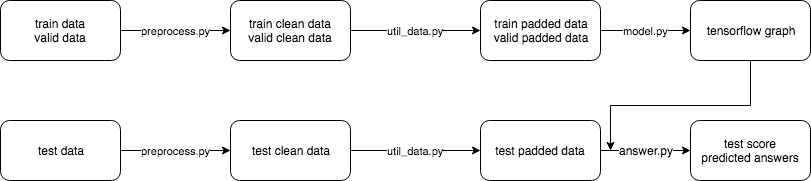
\includegraphics[width=9cm, height=2.5cm]{figures/pipeline.png}
    \end{center}
\end{frame}

\section{Experiments}

\begin{frame} \frametitle{Data}
    \begin{itemize}
        \item The Stanford Question Answering Dataset (SQuAD) is used to do experiments.
        \begin{table}[htbp]\centering
          \begin{tabular}{|r|l|} \hline
            Set Name & Number of Instances \\ \hline\hline
            Train & \ 78,839 \\
            Validation & \ 8,760 \\
            Test & \ 10,570 \\ \hline
          \end{tabular}
        \end{table}
        \item The pre-trained GloVe word feature vectors are used to initialize words.
    \end{itemize}
\end{frame}

\begin{frame}\frametitle{Data}
    \begin{center}
        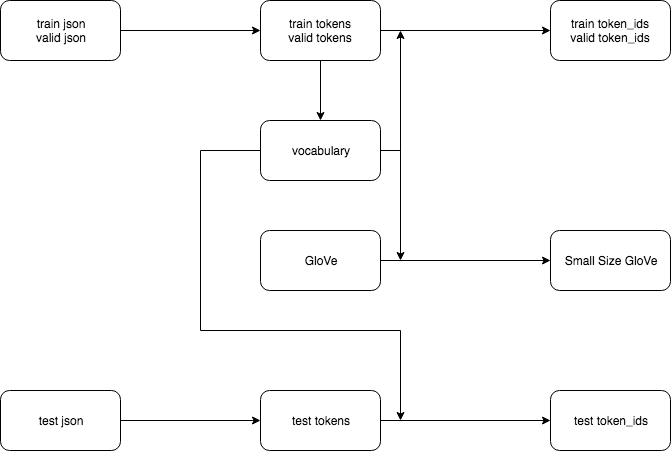
\includegraphics[width=8cm, height=6cm]{figures/data.png}
    \end{center}
\end{frame}

\begin{frame}{Settings}
    \begin{itemize}
        \item 400 is set as $passage\_padding\_length$
            \begin{center}
                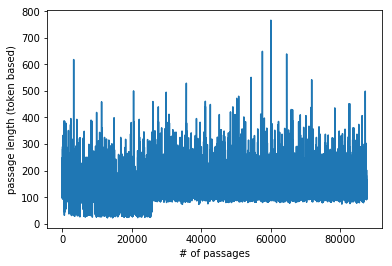
\includegraphics[width=6cm, height=4cm]{figures/passage_length.png}
            \end{center}
    \end{itemize}
\end{frame}

\begin{frame}{Settings}
    \begin{itemize}
        \item 30 is set as $question\_padding\_length$
            \begin{center}
                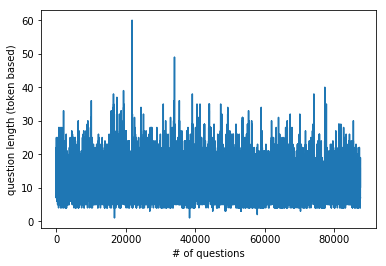
\includegraphics[width=6cm, height=4cm]{figures/question_length.png}
            \end{center}
    \end{itemize}
\end{frame}

\begin{frame}{Settings}
    \begin{itemize}
        \item The learning rate is set at 0.002 through experiments.
    \end{itemize}
    \begin{center}
        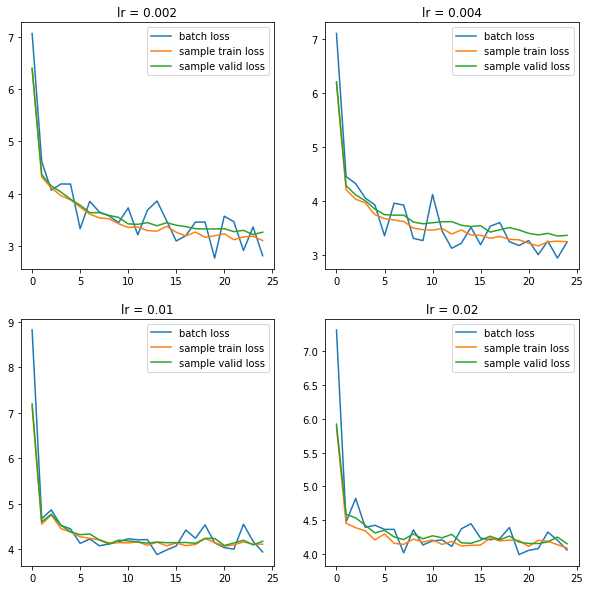
\includegraphics[width=7cm, height=7cm]{figures/lr.png}
    \end{center}
\end{frame}

\begin{frame}{Settings}
    \begin{table}[htbp]\centering

      \begin{tabular}{|r|l|} \hline
        Hyperparameter Name& Value \\ \hline\hline
        Word Feature Vector Dimension (d) & \ 100 \\
        Hidden State Size (l) & \ 64 \\
        L2\_regularization Scale & \ 0.001\\
        Hidden State Size (l) & \ 64\\
        Batch Size & \ 64\\
        Passage Length & \ 400\\
        Question Length & \ 30\\
        Clip Norm & \ 5\\
        Learning Rate & \ 0.002 \\ \hline
      \end{tabular}
    \end{table}
\end{frame}

\begin{frame}{Settings}
    \begin{itemize}
        \item The F1 score and the exact match score are used to evaluate the performance of each model.
            \begin{itemize}
                \item F1 treats a predicted answer and a ground truth as bag of words and calculate a harmonic average of precision and recall;
                \item exact match measures the percentage of predictions and ground truths that are exactly the same.
            \end{itemize}
        \item The testing data contains several ground truth answers for one passage-question pair. The best score is chosen as the final score.
        \item A machine that has Tesla K80 12 GB Memory, 61 GB RAM and 100 GB SSD is used to train the models.
    \end{itemize}
\end{frame}

\begin{frame}{Training Process}
    \begin{itemize}
        \item One epoch contains roughly 25 * 100 mini batches.
        \item The training loss and training scores are calculated every 100 mini batches using the 200 sample instances from training set. We do the same for validation loss and validation scores.
        \item Training one epoch takes roughly 100 minutes. A thorough training of each model requires around 10 epochs and takes around 17 hours.
    \end{itemize}
\end{frame}

\begin{frame}{Training Process}\framesubtitle{Model 1}
    \begin{center}
        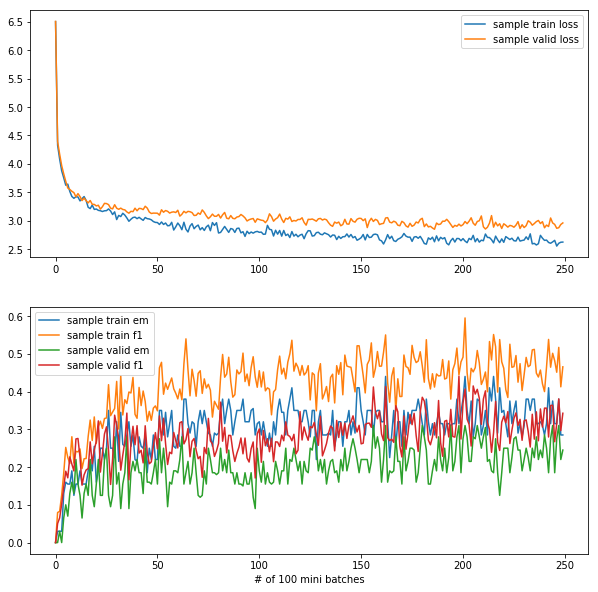
\includegraphics[width=8cm, height=7cm]{figures/match_corrected.png}
    \end{center}

\end{frame}

\begin{frame}{Training Process}\framesubtitle{Model 2}
    \begin{center}
        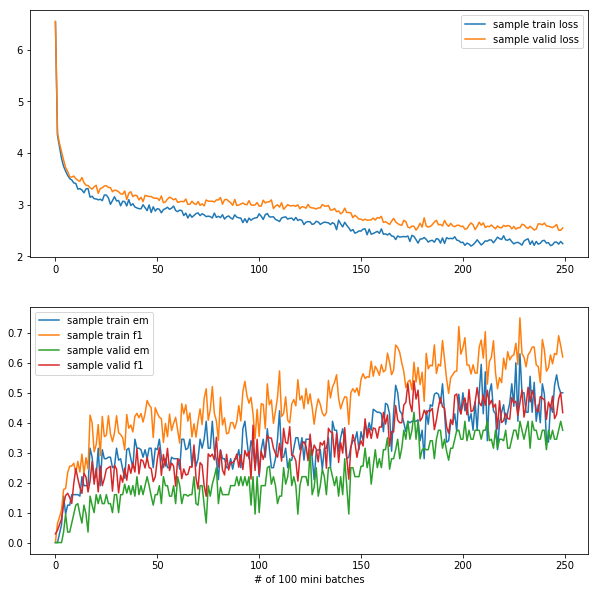
\includegraphics[width=8cm, height=7cm]{figures/match_baseline.png}
    \end{center}
\end{frame}

\begin{frame}{Training Process}\framesubtitle{Model 3}
    \begin{center}
        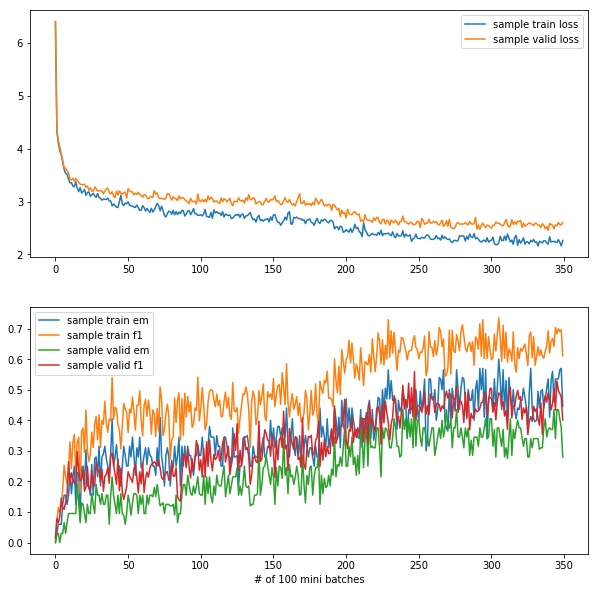
\includegraphics[width=8cm, height=7cm]{figures/match_change1.png}
    \end{center}

\end{frame}

\begin{frame}{Training Process}\framesubtitle{Model 4}
    \begin{center}
        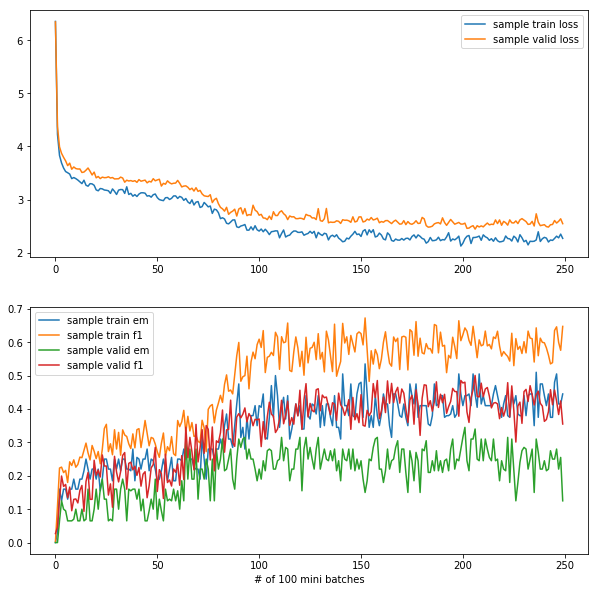
\includegraphics[width=8cm, height=7cm]{figures/match_change2.png}
    \end{center}

\end{frame}

\begin{frame}{Training Process}\framesubtitle{Model 5}
    \begin{center}
        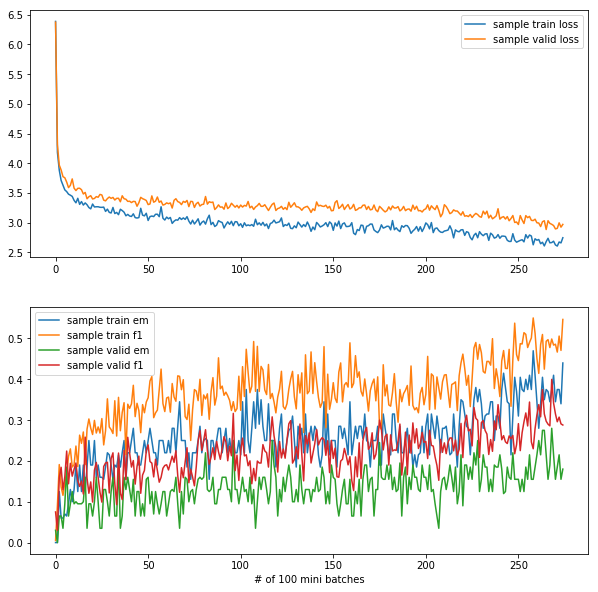
\includegraphics[width=8cm, height=7cm]{figures/match_change3.png}
    \end{center}

\end{frame}

\begin{frame}{Testing Results}
    \begin{table}[htbp]\centering
      \begin{tabular}{|c|c|c|}
        \hline
        Model& Test Exact Match & Test F1 \\
        \hline\hline
        Reference Paper & \ 64.7 &\ 73.7 \\
        Model 1 & \ 23.4 &\ 33.6 \\
        Model 2 & \ 33.0 &\ 45.8 \\
        Model 3 & \ 33.0 &\ 46.2 \\
        Model 4 & \ 33.0 &\ 45.6 \\
        Model 5 & \ 24.3 &\ 33.9 \\
        \hline
      \end{tabular}
    \end{table}
\end{frame}

\begin{frame}{Analysis}
    \begin{itemize}
        \item Model 1 didn't reproduce the results of the original paper.
        \item Model 2 has better score than Model 1. This indicates using attention vector to query attention weight might be better than using the LSTM state.
    \end{itemize}
\end{frame}

\begin{frame}{Analysis}
    \begin{itemize}
        \item Model 2, 3 and 4 have similar scores. This indicates either removing the preprocessing layer or not using LSTM state to query attention vector in the bidirectional match LSTM layer does not decrease test results.

        \item Model 5 performs worse than Model 2, 3 and 4. This means the change in Model 3 encoder and Model 4 encoder cannot be made together. A reasonable guess is the context information provided by these two parts is not provided in other parts of Model 2.
    \end{itemize}
\end{frame}

\section{Conclusion}

\begin{frame}{Contribution of This Project}
    \begin{itemize}
        \item This project presented a thorough implementation of a question answering system. \item Five different models were tried and several interesting observations were found.
    \end{itemize}

\end{frame}

\begin{frame} \frametitle{Future Work}
    \begin{itemize}
        \item Further work is required to find out why Model 1 failed to reproduce the testing results of the reference paper.
        \item At the same time, more parameter tuning work is required to make the experiments more precise. \item Last but not the least, making novel architectures to bypass the state-of-art results is always a good way to move the question answering research forward.
    \end{itemize}
\end{frame}

\begin{frame}
Thank you! Questions?
\end{frame}

\end{document}
